%% Based on a TeXnicCenter-Template, which was
%% created by Christoph B�rensen
%% and slightly modified by Tino Weinkauf.
%%%%%%%%%%%%%%%%%%%%%%%%%%%%%%%%%%%%%%%%%%%%%%%%%%%%%%%%%%%%%
\documentclass[a4paper,abstracton]{scrartcl}
%########################### Preferences #################################


% ******** vmargin settings *********
\usepackage{vmargin} %This give you full control over the used page arae, it maybe not the idea od Latex to do so, but I wanted to reduce to amount of white space on the page
\setpapersize{A4}
\setmargins{3.5cm}%			%linker Rand, left edge
					 {1.5cm}%     %oberer Rand, top edge
           {14.7cm}%		%Textbreite, text width
           {23.42cm}%   %Texthoehe, text hight
           {14pt}%			%Kopfzeilenh�he, header hight
           {1cm}%   	  %Kopfzeilenabstand, header distance
           {0pt}%				%Fu�zeilenhoehe footer hight
           {2cm}%    	  %Fusszeilenabstand, footer distance         

% ********* Font definiton ************
\usepackage{t1enc} % as usual
\usepackage[latin1]{inputenc} % as usual
\usepackage{times}		
%\usepackage{mathptmx}  	%mathematical fonts for use with times, I encountered some problems using this package togather with pdftex, which I was not able to resolve

% ********* Graphics definition *******
\usepackage[pdftex]{graphicx} % required to import graphic files
\usepackage{color} %allows to mark some entries in the tables with color
\usepackage{eso-pic} % these two are required to add the little picture on top of every page
\usepackage{everyshi} % these two are required to add the little picture on top of every page
\renewcommand{\floatpagefraction}{0.7} %default:0.5 allows two big pictures on one page

%********** Enybeling Hyperlinks *******
\usepackage[pdfborder=000,pdftex=true]{hyperref}% this enables jumping from a reference and table of content in the pdf file to its target

% ********* Table layout **************
\usepackage{booktabs}	  	%design of table, has an excellent documentation
%\usepackage{lscape}			%use this if you want to rotate the table together with the lines around the table

% ********* Caption Layout ************
\usepackage{ccaption} % allows special formating of the captions
\captionnamefont{\bf\footnotesize\sffamily} % defines the font of the caption name (e.g. Figure: or Table:)
\captiontitlefont{\footnotesize\sffamily} % defines the font of the caption text (same as above, but not bold)
\setlength{\abovecaptionskip}{0mm} %lowers the distace of captions to the figure


% ********* Header and Footer **********
% This is something to play with forever. I use here the advanced settings of the KOMA script

\usepackage{scrpage} %header and footer using the options for the KOMA script
\renewcommand{\headfont}{\footnotesize\sffamily} % font for the header
\renewcommand{\pnumfont}{\footnotesize\sffamily} % font for the pagenumbers

%the following lines define the pagestyle for the main document
\defpagestyle{cb}{%
(\textwidth,0pt)% sets the border line above the header
{\pagemark\hfill\headmark\hfill}% doublesided, left page
{\hfill\headmark\hfill\pagemark}% doublesided, right page
{\hfill\headmark\hfill\pagemark}%  onesided
(\textwidth,1pt)}% sets the border line below the header
%
{(\textwidth,1pt)% sets the border line above the footer
{{\it Federation Confidential}\hfill Chief O'Brian}% doublesided, left page
{Chief O'Brian\hfill{\it Federation Confidential}}% doublesided, right page
{Chief O'Brian\hfill{\it Federation Confidential}} % one sided printing
(\textwidth,0pt)% sets the border line below the footer
}

%this defines the page style for the first pages: all empty
\renewpagestyle{plain}%
	{(\textwidth,0pt)%
		{\hfill}{\hfill}{\hfill}%
	(\textwidth,0pt)}%
	{(\textwidth,0pt)%	
		{\hfill}{\hfill}{\hfill}%
	(\textwidth,0pt)}

%********** Footnotes **********
\renewcommand{\footnoterule}{\rule{5cm}{0.2mm} \vspace{0.3cm}} %increases the distance of footnotes from the text
\deffootnote[1em]{1em}{1em}{\textsuperscript{\normalfont\thefootnotemark}} %some moe formattion on footnotes

%################ End Preferences, Begin Document #####################

\pagestyle{plain} % on headers or footers on the first page




%%%% my stuff (habi)

\usepackage[ansinew]{inputenc}
\usepackage[small,bf,hang]{caption}
\usepackage[format=hang]{subfig}
\usepackage[disable]{todonotes} % disable
\usepackage{graphicx}
\usepackage{natbib}
\usepackage{SIunits}
\usepackage{url}
\usepackage{hyperref}
\usepackage{tikz}
\usetikzlibrary{shapes,arrows}

\usepackage[T1]{fontenc}
\usepackage{lmodern}
\usepackage{mathpazo}
\usepackage{helvet} 

\newcommand{\imsize}{.618\textwidth}

\title{Wide Field Scan Paper}
\author{David Haberth�r, Christoph Hinterm�ller, Johannes Schittny, Marco Stampanoni}

\begin{document}
\maketitle

\listoftodos
\begin{abstract}
abstract
\end{abstract}
%!TEX root = widefieldscan.tex
\svnidlong
{$HeadURL$}
{$LastChangedDate$}
{$LastChangedRevision$}
{$LastChangedBy$}

\begin{center}
	\fbox{
		\begin{minipage}{.618\columnwidth}
		The section below is versioned at \url{\svnkw{HeadURL}} (last commit @ \svnfileday.\svnfilemonth.\svnfileyear \space \svnfilehour:\svnfileminute, Revision: \svnkw{LastChangedRevision}).
		\end{minipage}
	} 
\end{center}

\section{Introduction}
Synchrotron radiation based x-ray tomographic microscopy (SRXTM) is a powerful method for the non-destructive three-dimensional imaging of a broad kind of materials with a resolution on the sub-micrometer scale.

At TOMCAT---the beamline for TOmographic Microscopy and Coherent rAdiology experimenTs~\cite{Stampanoni2007} at the Swiss Light Source (SLS), Paul Scherrer Institute, Villigen, Switzerland---more than 20 user groups are presently working in diverse research areas, ranging from biology, medicine and paleontology to materials science, geology and process engineering\todo{citations?}. SRXTM enables the user to have a qualitative and quantitative measurement and analysis of nearly any structure.

\subsection{Background}
Various applications depend on the availability of high resolution tomographic images of the studied sample. The available field of view (FOV) of microscopy based imaging methods like synchrotron based tomographic beam lines and micro-computed tomography (\micro CT) stations is limited by the camera and microscope optics. To be able to obtain images with a broad FOV one has to use lower magnifications to cover bigger samples.

To record tomographic datasets at TOMCAT with a resolution of around \SI{1}{\micro\meter}, the sample diameter has to be below \SI{1}{\milli\meter}. This constraint can be overcome with so called local tomography, where the sample diameter is bigger than the FOV, but this a) introduces image artifacts at the edges of the reconstructed slices and b) does not solve the need for tomographic datasets with high resolution and large lateral FOV.

\subsection{Motivation}
\label{subsec:motivation}
At our group we have been studying lung development~\cite{Schittny2008,Mund2008} and lung structure~\cite{Tsuda2008} using SRXTM. Until now, the investigation of the three dimensional structure of an entire acinus---the functional lung unit---was either limited by the resolution of the imaging method (in the case of \micro CT) or the sample volume (in the case of SRXTM). We developed a synchrotron radiation x-ray tomographic microscopy method to combine several tomographic scans into one large three dimensional dataset to increase the scanned volume by a factor of nine in the simple and up to a factor of 25 in the advanced case.

\subsection{Enhancing the Field of View}
\label{subsec:enhancing the field of view}
An increase of the FOV parallel to the rotation axis of the sample can be achieved through the stacking of multiple scans on top of each other. This stacking has been implemented at TOMCAT through accurately controlling the end-station setup and sample position.

This means that the final reconstructions can simply be stacked on top of each other, even if they have been acquired in different scans. For this imaging mode, the scanning time linearly increases with the sample size.

If the FOV horizontal to the rotation axis of the sample is to be increased, the projections cannot simply be merged together, since the sampling theorem implies some restrictions, which are detailed below.

Generally, to be able to accurately reconstruct a sample, we have to fulfill the sampling theorem for computed tomography. \citet{Kak2002} stated that for parallel beam tomography: \begin{quote} The number of projections should be roughly equal to the number of rays in each projection. \end{quote} In our case the number of rays corresponds to the amount of pixels for the width of the detector, thus equals 2048 pixels. The precondition can be slightly violated, with the result that at TOMCAT, for an un-binned scan---which equals a detector width of 2048 pixels---1500 projection images are obtained for a sample rotation over \SI{180}{\degree}. In the binned case---where 2$\times$2 pixels are combined into one pixel, equaling a detector width of 1024 pixels---1000 projection images are recorded for one tomographic scan.

If we thus aim to enlarge the FOV of the tomographic images perpendicular to the rotation axis of the sample, it is not only necessary to stitch together several projection images, but it is also necessary to record more projections for the lateral parts of the sample compared to the central parts of the sample to be able to fulfill the sampling theorem. This leads to an increase in imaging and post-processing time as compared to a standard scan with a comparably smaller FOV. Let us assume that we have a sample that could be imaged using three overlapping FOVs of 1024 pixels, we have to obtain approximately 3000 projections in the lateral parts of the sample to fulfill the aforementioned sampling theorem\todo{Do we need to explain the sampling theorem in more depth?}.

During the development of the scanning protocols for the wide field scanning, we have seen that a small overlapping region between the separate subscans is necessary to be able to correctly stitch the single projection images from the subscans into one big projection (see section~\ref{subsec:covering a broad fov} for details). TOMCAT has the possibility to operate in the so called \SI{360}{\degree} mode, where a sample is scanned with full a full rotation, while the camera window only covers half of the sample dimensions (see figure~\ref{subfig:scanning-possibilities} for details). Afterwards, the projections are automatically stitched together and a full projection is formed. Preliminary results have shown, that using this \SI{360}{\degree}-scanning method was not viable for performing the wide field scans, even with precise calibration the outer scans could not be stitched together without introducing errors in the reconstruction. We would also have needed to introduce more processing steps like flipping of the projection images obtained in the second half of the rotation prior to stitching, so that we chose to only perform \SI{180}{\degree}-scans, but overlapping in such a sense that the outcome is equivalent to scanning with the \SI{360}{\degree}-method, except the projection images are obtained at three instead of two positions.

If we want to stitch together multiple subscans, \todo{sub scan, sub-scan or subscan?} we have to keep in mind that do not record an equal amount of projections for each of the subscans and thus need to make sure the stitching and concatenation into projections covering the desired full FOV is correctly performed.

\begin{figure*}
	\centering
		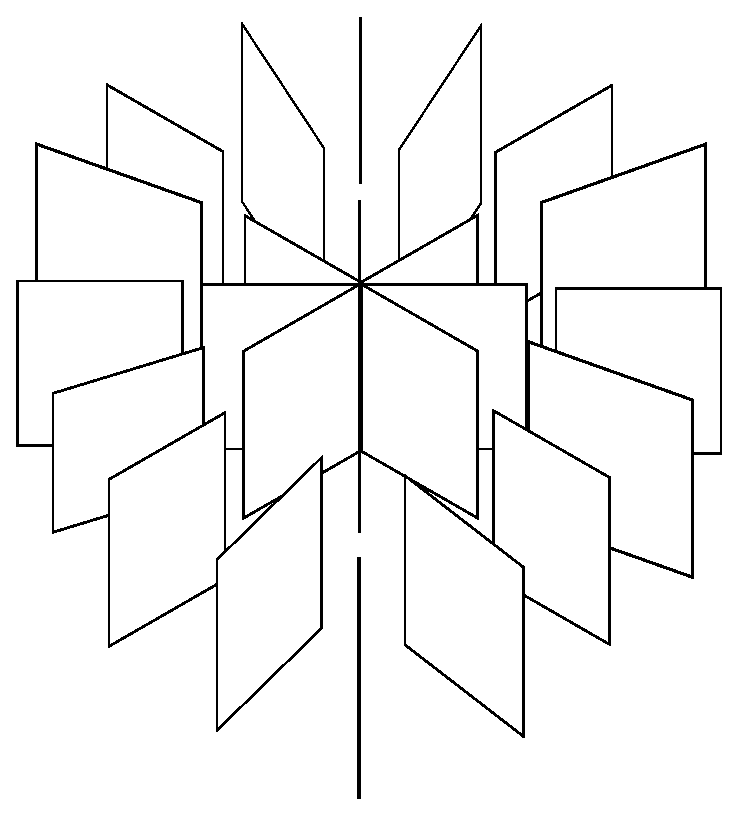
\includegraphics[width=\imsize]{img/projections}
	\caption{Projection Setup with one central and one ring-scan. For demonstration purposes, the central scan has four projections and the ring scan has 16 projections over \SI{360}{\degree}. This is essentially the same as two \SI{180}{\degree}-scans with eight projections each.}
	\label{fig:projections}
\end{figure*}

%!TEX root = widefieldscan.tex
\section{Materials and Methods}

\footnote{Author: \svnauthor; Revision: \svnrev; Last changed on: \svndate; URL: \url{\svnkw{HeadURL}}}

\subsection{TOMCAT}
here we should describe TOMCAT
\subsubsection{Sample Stage}
how is the stuff moving?

\svnidlong
{$HeadURL$}
{$LastChangedDate$}
{$LastChangedRevision$}
{$LastChangedBy$}
\framebox{Author: \svnauthor; Rev: \svnrev; Last change: \svndate}% - URL: \url{\svnkw{HeadURL}}}
\section{Results}
Results of the aforementioned steps are shown in figure~\ref{fig:wide field scan}. Figure~\ref{subfig:wfs-sub} shows exemplary projection images from overlapping subscans prior to correction and normalization. Figure~\ref{subfig:wfs-mrg} shows a merged projection image prior to reconstruction and figure~\ref{subfig:wfs-slice} shows the end-result of such a wide field scan, a reconstructed slice of the whole sample with a FOV of \unit{5.734}{\milli\meter} --- approximately five times the size of what can be achieved with one single scan.
\begin{figure}[p] % [tb] for small, [p] for big pictures
	\centering
	\begin{minipage}{0.66\textwidth}
	\renewcommand{\imsize}{0.2\textwidth}
	\subfloat[Raw projection images from five overlapping subscans. Each image has an original size of 1024$\times$1024 pixels and covers a FOV of approximately \unit{0.7}{\milli\meter}. The images have been rescaled to 512$\times$512 pixels for display purposes.]{\label{subfig:wfs-sub}\includegraphics[width=\imsize]{mrg/R108C04BrulW-s10444}\includegraphics[width=\imsize]{mrg/R108C04BrulW-s20444}\includegraphics[width=\imsize]{mrg/R108C04BrulW-s30444}\includegraphics[width=\imsize]{mrg/R108C04BrulW-s40444}\includegraphics[width=\imsize]{mrg/R108C04BrulW-s50444}}\\
	\renewcommand{\imsize}{\textwidth}
	\subfloat[Merged and corrected projection composed from the subscans shown in \subref{subfig:wfs-sub}. The merged projection has a size of 4502$\times$1024 pixels. The scans shown above overlap each other by 15\%, approximately 150 pixels. A slice reconstructed from a set of merged projections like the one shown here is shown in \subref{subfig:wfs-slice}. The image has been rescaled to 2251$\times$512 pixels for display purposes.]{\label{subfig:wfs-mrg}\includegraphics[width=\imsize]{mrg/R108C04BrulW-cnc0444}}\\
	\subfloat[Reconstructed slice of the full data set with a size of 8192$\times$8192 pixels, covering a FOV of approximately \unit{5.75}{\milli\meter}. The Image has been rescaled to 1024$\times$1024 pixels for display purposes.]{\label{subfig:wfs-slice}
\includegraphics[angle=90,width=\imsize]{R108C04BrulW-1001-mrg-orig}}\\
	\caption{Different stages of a wide field scan of a sample obtained from a Sprague-Dawley rat 4 days after birth, scanned at a beam energy of \unit{12.6}{\kilo\electronvolt}.}	
	\label{fig:wide field scan}
	\end{minipage}
\end{figure}

%!TEX root = widefieldscan.tex
\svnidlong
{$HeadURL$}
{$LastChangedDate$}
{$LastChangedRevision$}
{$LastChangedBy$}
%
%\ifhtml
%\else
%\begin{center}
%	\fbox{
%		\begin{minipage}{.618\columnwidth}
%		The section below is versioned at \url{\svnkw{HeadURL}} (last commit @ \svnfileday.\svnfilemonth.\svnfileyear \space \svnfilehour:\svnfileminute, Revision: \svnkw{LastChangedRevision}).
%		\end{minipage}
%	} 
%\end{center}
%\fi
%
\section{Discussion}
\label{sec:Discussion}
We present a method to increase the field of view of parallel beam tomographic imaging methods\todo{discuss what happens for cone-beam - marco?} and would like to call this method wide field synchrotron radiation based x-ray tomographic microscopy (WF-SRXTM). We selectively defined different scanning protocols for the optimization of the total imaging time towards the expected imaging quality. This enables the very fast acquisition of lower quality tomographic datasets or acquisition of very high quality datasets in a longer time.

The field of view was increased three-fold by merging projections from three subscans and reconstructing the merged projections using the standard workflow present at the beamline. As a consequence of increasing the field of view, an increased amount of projections have to be acquired to satisfy the sampling theorem. This increased amount of projections lengthens the acquisition time. To overcome this limitation, we defined multiple scanning protocols with a reduced amount of total projections. All these protocols have been evaluated for quality of the resulting reconstructions compared to a gold standard. We have shown that the resulting quality can be simulated prior to scanning, thus giving the end-user a possibility to chose a suited scanning protocol, based on needed scanning time and on an estimation of the quality of the resulting reconstructions.

For protocols with an equal amount of total projections, but differing amount of projections for the central and the ring scans we observed a difference in reconstruction quality (protocols C and D as well as protocols M and N are such protocols and are marked in figure~\ref{fig:NormalizedErrorPlot}). Such a difference arises through the fact that the amount of projections acquired for the central and the subscan do add up to the same total amount of projections, but contribute differently to the quality of the reconstruction. Two factors are responsible for this result: First, we perform an oversampling in the central scan for both protocols D and N when compared to protocols C and M, which increases the quality of the reconstructions. Second, since we acquired different amount of projections for the subscans, we need to interpolate projections from the central scan to generate merged projections, which accounts for an additional error for protocols M and C\todo{Additionally a ``missing wedge''-problem for outer scans?}.

It is thus desirable to favor a protocol with equal amounts of projections for each subscans over of a protocol with an equal total amount of projections, but a decreased amount of projections for the central scan. Since a reduced amount of projections for the central scan decrease the reconstruction quality for the central parts of the sample, this explanation seems natural. In addition, the interpolation of missing projections could introduce artifacts in the reconstruction which are suppressed when simply stitching projections without interpolation.

We have shown that the field of view of parallel beam tomographic end-stations can be increased up to five-fold and have three-dimensionally reconstructed multiple tomograms obtained with WF-SRXTM. The calculation shown for three subscans (one central and two half ring scans) are expandable to 5 subscans, as has been shown at the end of section~\ref{sec:Results}. The protocols are theoretically expandable for more than the shown 5 subscans, albeit the reconstruction of wide field scans with 7 or more subscans implies tremendous requirements on the data processing infrastructure. The datasets shown in figure~\ref{fig:BvsT} are binned scans resulting in datasets of 1024 slices, each with a size of 2792$\times$2792 pixels at a \SI{8}{\bit} depth. This amounts to a total size of the dataset of approximately \SI{7.5}{\giga\byte}. If we assume an un-binned scan with 7 overlapping subscans, the size of the stitched projections will be around 14000$\times$14000 pixels. The full dataset will consist of 2048 stitched slices with that size, with amounts to a total size of approximately \SI{383}{\giga\byte} for the full dataset. All mentioned datasets have been reconstructed at \SI{8}{\bit}, TOMCAT also offers the possibility to record the tomographic datasets with \SI{16}{\bit} depth, so the full dataset of a wide field scan with a seven-fold increase in field of view with increased bit depth would result in one dataset with a size of \SI{0.75}{\tera\byte}.

Nonetheless the scanning of samples with a five-fold increase in field of view or bigger is interesting, since it would enable the end-user to selectively reconstruct regions of interest (ROI) from large samples with ultra-high resolution. Up to now a two-step process was required to scan ROI from samples larger than the field of view at the high resolution. In a first step, a registered overview scan of the sample at lower resolution and thus large field of view was acquired, then a ROI to be scanned with high resolution was defined in this low-resolution tomographic dataset using a custom-made ROI picker software~\cite{Heinzer2008} and a high resolution local tomography scan with low field of view of this selected ROI was performed at a second allotted beam shift at TOMCAT. This cumbersome two-step process now only has to be used in the case where the highest possible resolution and contrast are required and the limitation in field of view is not important.

One disadvantage of WF-SRXTM compared to the ROI picker method is the extremely big datasets which resulting from the reconstruction of the full resolution projections into reconstructions spanning a large field of view. With the ROI picker method only selective regions of interest selected from a low-resolution tomogram are scanned and reconstructed in high resolution. Since we record all data in a one-step process, it would be possible to integrate partial reconstructions of the full size datasets into the data processing pipeline of TOMCAT. After definition of a ROI to be reconstructed out of the high-resolution wide field dataset, partial sinograms and partial reconstructions could be calculated.
% !TEX root = widefieldscan.tex
\svnidlong
{$HeadURL: http://code.ana.unibe.ch/svn/WideFieldScanPaper/pre213wfs-summary.tex $}
{$LastChangedDate: 2010-01-08 17:25:03 +0100 (Fr, 08 Jan 2010) $}
{$LastChangedRevision: 214 $}
{$LastChangedBy: $}
%
\section{Summary}\label{summary}

A method to increase the lateral field of view of tomographic imaging has been established, which enables the high-resolution tomographic imaging of large samples that are wider than the field of view of the optical setup in multiple semi-automatically combined steps. Tomographic datasets of entire rat lung acini have been acquired with an enhanced field of view using WF-SRXTM.

Different optimized scanning protocols for covering a large field of view have been validated and are now provided for the end-users of the TOMCAT beamline. End-users now have the possibility to choose suitable scanning protocols depending on a balance between acquisition time and expected reconstruction quality. Depending on this balance, a reduction of the image acquisition time by \SI{84}{\percent} is possible, while keeping the quality of the reconstructed tomographic dataset on a level still permitting automated segmentation of the lung structure and surrounding airspace, as shown in section~\ref{subsec:comparison}. The reduction in acquisition time obviously reduces the time during which the sample is irradiated by synchrotron radiation and thus reduces the radiation dose inflicted on the sample.
%!TEX root = widefieldscan.tex
\svnidlong
{$HeadURL$}
{$LastChangedDate$}
{$LastChangedRevision$}
{$LastChangedBy$}

\section{Acknowledgements}
\footnote{Author: \svnauthor; Rev: \svnrev; Last change: \svndate}% - URL: \url{\svnkw{HeadURL}}}
\begin{itemize}
	\item Chrigu Lehmann - sample preparation for the first samples
	\item Federica Marone - help at the beamline
	\item SNF grant Nr. (David)
	\item NASA grant Nr. (Chris)
\end{itemize}

\bibliographystyle{unsrt}
\bibliography{../references}

\end{document}



